
\documentclass[useAMS,usenatbib,article]{mn2e}

\usepackage{longtable}
\usepackage[]{graphicx}
\usepackage{amsmath}
\usepackage{natbib}
\bibliographystyle{mn2e}
%\usepackage{tabularx}
%\usepackage{bm}
%\usepackage{color}
%\usepackage{hyperref}

%% Sometimes a paper's abstract is too long to fit on the
%% title page in preprint2 mode. When that is the case,
%% use the longabstract style option.

%% \documentclass[preprint2,longabstract]{aastex}
\newcommand\aj{{AJ}}%
\newcommand\actaa{{Acta Astron.}}%
\newcommand\araa{{ARA\&A}}%
\newcommand\apj{{ApJ}}%
\newcommand\apjl{{ApJ}}%
\newcommand\apjs{{ApJS}}%
\newcommand\ao{{Appl.~Opt.}}%
\newcommand\apss{{Ap\&SS}}%
\newcommand\aap{{A\&A}}%
\newcommand\aapr{{A\&A~Rev.}}%
\newcommand\aaps{{A\&AS}}%
\newcommand\azh{{AZh}}%
\newcommand\baas{{BAAS}}%
\newcommand\caa{{Chinese Astron. Astrophys.}}%
\newcommand\cjaa{{Chinese J. Astron. Astrophys.}}%
\newcommand\icarus{{Icarus}}%
\newcommand\jcap{{J. Cosmology Astropart. Phys.}}%
\newcommand\jrasc{{JRASC}}%
\newcommand\memras{{MmRAS}}%
\newcommand\mnras{{MNRAS}}%
\newcommand\na{{New A}}%
\newcommand\nar{{New A Rev.}}%
\newcommand\pra{{Phys.~Rev.~A}}%
\newcommand\prb{{Phys.~Rev.~B}}%
\newcommand\prc{{Phys.~Rev.~C}}%
\newcommand\prd{{Phys.~Rev.~D}}%
\newcommand\pre{{Phys.~Rev.~E}}%
\newcommand\prl{{Phys.~Rev.~Lett.}}%
\newcommand\pasa{{PASA}}%
\newcommand\pasp{{PASP}}%
\newcommand\pasj{{PASJ}}%
\newcommand\qjras{{QJRAS}}%
\newcommand\rmxaa{{Rev. Mexicana Astron. Astrofis.}}%
\newcommand\skytel{{S\&T}}%
\newcommand\solphys{{Sol.~Phys.}}%
\newcommand\sovast{{Soviet~Ast.}}%
\newcommand\ssr{{Space~Sci.~Rev.}}%
\newcommand\zap{{ZAp}}%
\newcommand\nat{{Nature}}%
\newcommand\iaucirc{{IAU~Circ.}}%
\newcommand\aplett{{Astrophys.~Lett.}}%
\newcommand\apspr{{Astrophys.~Space~Phys.~Res.}}%
\newcommand\bain{{Bull.~Astron.~Inst.~Netherlands}}%
\newcommand\fcp{{Fund.~Cosmic~Phys.}}%
\newcommand\gca{{Geochim.~Cosmochim.~Acta}}%
\newcommand\grl{{Geophys.~Res.~Lett.}}%
\newcommand\jcp{{J.~Chem.~Phys.}}%
\newcommand\jgr{{J.~Geophys.~Res.}}%
\newcommand\jqsrt{{J.~Quant.~Spec.~Radiat.~Transf.}}%
\newcommand\memsai{{Mem.~Soc.~Astron.~Italiana}}%
\newcommand\nphysa{{Nucl.~Phys.~A}}%
\newcommand\physrep{{Phys.~Rep.}}%
\newcommand\physscr{{Phys.~Scr}}%
\newcommand\planss{{Planet.~Space~Sci.}}%
\newcommand\procspie{{Proc.~SPIE}}%


%\newcommand{\vdag}{(v)^\dagger}
%\newcommand{\myemail}{gsavorgn@astro.swin.edu.au}
%\newcommand{\fitfigurewidth}{0.8\textwidth}


%\title[Intermediate-scale discs]{Early-type galaxies with intermediate-scale discs and their ordinary supermassive black holes}
\title[Ellicular galaxies]{Ellicular galaxies and their (non {\"u}ber-massive) black holes}


\author[G.~A.~D. Savorgnan \& A.~W. Graham]
{\parbox{\textwidth}{
Giulia~A.~D. Savorgnan$^{1}$\thanks{E-mail: \texttt{gsavorgn@astro.swin.edu.au}},
Alister W. Graham$^{1}$}\vspace{0.4cm}\\
\parbox{\textwidth}{
$^{1}$Centre for Astrophysics and Supercomputing, Swinburne University of Technology, Hawthorn, Victoria 3122, Australia.\\}}

\pagerange{\pageref{firstpage}--\pageref{lastpage}} \pubyear{2015}

\begin{document}

\maketitle

\label{firstpage}



\begin{abstract}
The classification early-type galaxy includes both elliptically-shaped and lenticular galaxies, 
with the latter composed of a spheroid, or bulge, of stars encased within a larger, but flatter, stellar disc. 
Theoretically, the spheroid-to-disc flux ratio can assume any positive value. 
However, several studies only consider spheroid/disc decompositions 
in which the disc neatly dominates over the spheroid at large galaxy radii -- creating an inner bulge -- 
and they reject decompositions if the disc remains embedded within the spheroid, labeling them as ``unphysical''. 
Here we show that these rejected models correctly reproduce the photometric and kinematic properties of a class of early-type galaxy 
%with intermediate-scale disc. 
%Intermediate-scale discs have often been confused with large-scale discs, 
%and as a consequence the disc luminosities have been considerably overestimated 
%and their spheroid luminosities underestimated. 
intermediate between that of elliptical and lenticular galaxies, and which we name ellicular galaxies. 
Ellicular galaxies have often been confused with lenticular galaxies, and as a consequence their disc luminosities have been considerably overestimated 
and their spheroid luminosities underestimated. 
This has recently led to some surprising conclusions, 
such as the claim that a number of ellicular galaxies (Mrk 1216, NGC 1277, NGC 1271, and NGC 1332) 
host a central black hole whose mass is abnormally large compared to expectations from the (underestimated) spheroid luminosity. 
When ellicular galaxies are properly modeled, 
they no longer appear as extreme outliers in the (black hole mass)-(spheroid mass) diagram, 
thereby resolving previous anomalies. 
This not only nullifies the need for invoking different evolutionary scenarios for these galaxies 
but it strengthens the significance of the observed (black hole mass)-(spheroid mass) correlation 
and confirms its importance as a fundamental ingredient for theoretical and semi-analytic models 
used to describe the coevolution of spheroids and their central supermassive black holes. 

\end{abstract}

\begin{keywords}
black hole physics -- galaxies: bulges -- galaxies: elliptical and lenticular, cD -- galaxies: evolution -- galaxies: structure
\end{keywords}

\section{Introduction}
\label{sec:int}
There are currently two well-known types of stellar discs in galaxies. 
The first are the large-scale discs (with sizes of a few kiloparsec) 
that dominate the light at large radii in spiral and lenticular galaxies; 
the second are the small (tens to a couple of hundred parsec) nuclear discs observed in both early- and late-type galaxies 
(e.g.~\citealt{scorzavandenbosch1998,rest2001,balcells2007,ledo2010}). 
The origin of the nuclear discs has been speculated to arise from the infall of small satellite galaxies or gas clouds.  
The origin, or at least the on-going feeding and growth, of the large-scale discs has been attributed to cold gas flows, 
gas rich mergers and halo accretion events 
(e.g.~\citealt{khochfarsilk2006,dekel2009nat,ceverino2010,ceverino2012,conselice2012}). 
A thorough review can be found in \citet{combes2014arX,combes2014pro}.
On the other hand, intermediate-sized discs have not received the same level of attention 
as their nuclear and large-scale homologues and,  
in some cases, they have even been labelled as something ''unphysical''. 
Here we report on the photometric and kinematical signatures of these intermediate-sized stellar discs 
and the impact this has on the important (black hole mass)-to-(spheroid stellar mass) ratio %, $M_{\rm BH}/M_{*,sph}$, 
which is used to constrain galaxy evolution models. \\
%A puzzling question, which has been unspoken for decades, is why are there not intermediate-sized discs: 
%why are there not accretion events which create discs larger than the typical nuclear discs but which are not large enough to dominate at large radii? 
The majority of stellar discs have some level of inclination with respect to our line-of-sight, 
and this makes them appear elliptical (rather than round) when seen in projection on the sky. 
This can help one distinguish them from the more spherically-shaped spheroids. 
Identifying the extent of these discs with respect to their spheroid can however be subtle. 
Two-dimensional kinematic maps represent an important diagnostic tool for this purpose. 
Most early-type galaxies are classified as ``central fast rotators'' \citep{atlas3dIII-MNRAS}, 
that is, they are rapidly rotating within their half-light radius.  
However, more extended kinematic maps \citep{arnold2014} reveal that 
some of the central fast rotators continue to be fast rotating at large radii, 
whereas other central fast rotators become slow rotators in their outer regions.
On the one hand, a specific angular momentum profile that is rapidly increasing beyond $1-2$ half-light radii 
is a signature of a large-scale disc. 
On the other hand, a specific angular momentum profile that increases up to $1-2$ half-light radii and declines beyond that point 
indicates the presence of an intermediate-scale disc that no longer dominates at large radii. 
Unfortunately, such extended kinematic maps are not yet available for large numbers of galaxies in the local Universe. 
Nevertheless, the ellipticity profile of a galaxy's isophotes can help identify the extent of stellar discs in early-type galaxies. \\
The toy model shown in Figure \ref{fig:model} illustrates the typical ellipticity profile 
($\epsilon = 1 - b/a$, where $b/a$ is the ratio of minor-to-major axis length) of 
(i) a lenticular galaxy, comprised of a large-scale disc and a relatively smaller encased bulge, 
(ii) an elliptical galaxy with a nuclear stellar disc, 
and (iii) a galaxy composed of an intermediate-scale disc embedded in a relatively larger spheroid. 
We refer to the last case as an ellicular galaxy. 
In general, stellar discs are intrinsically flat and circular; 
their ellipticity, dictated by their inclination to our line of sight, is fixed. 
Spheroids are often rounder than the observed projection on the sky of their associated discs, 
thus their average ellipticity is often lower than that of their disc. 
An ellipticity profile that increases with radius can be ascribed to an inclined disc that becomes progressively more important at large radii, 
whereas a radial decrease of ellipticity signifies the opposite case. \\
The awareness that many ``elliptical'' galaxies actually contain embedded stellar discs 
dates back at least three decades 
\citep{capaccioli1987,carter1987,rixwhite1990,bender1990,scorzabender1990,nieto1991,rixwhite1992,scorzabender1995,
donofrio1995,graham1998fornax,scorza1998,scorzavandenbosch1998} and, 
more recently, intermediate-scale discs were all but unfamiliar to \cite{kormendybender2012} and \cite{krajnovic2013etal}. 
However, the class of ellicular galaxies has been missed by many galaxy modellers, 
who have labelled as ``unphysical'' \citep{allen2006} those spheroid/disc decompositions in which the disc does not dominate over the spheroid at large radii 
as is observed with spiral galaxies. 
This unspoken bias has led to the rejection of many spheroid/disc decompositions similar to that illustrated in the middle panel of Figure \ref{fig:model}. 
Unsurprisingly, studies affected by this bias have not obtained spheroid/disc decompositions with a spheroid-to-total ratio larger than $0.6 - 0.8$ 
(e.g.~\citealt{gadotti2008,head2014,querejeta2015,mendezabreu2015}). \\
The existence of intermediate-scale stellar discs reveals a continuum of disc sizes, 
rather than a dichotomy of nuclear versus large-scale discs. 
The presence of intermediate-scale discs also blurs the distinction between elliptical and lenticular galaxies 
and creates the need for a new subclass to help bridge the divide. 
The existence of such discs is not only important for our understanding of disc growth in general, 
but accounting for such structure will impact our understanding of galaxy structure, 
with important consequences for galaxy scaling relations. 
%It has recently been argued that the classification scheme for elliptical galaxies should not be their apparent axis ratio as seen on the plane of the sky, 
%but instead their spheroid-to-total ratio, with a continuum from pure elliptical galaxies to disc-dominated lenticular galaxies \citep{graham2014review}.

\begin{figure}
\begin{center}
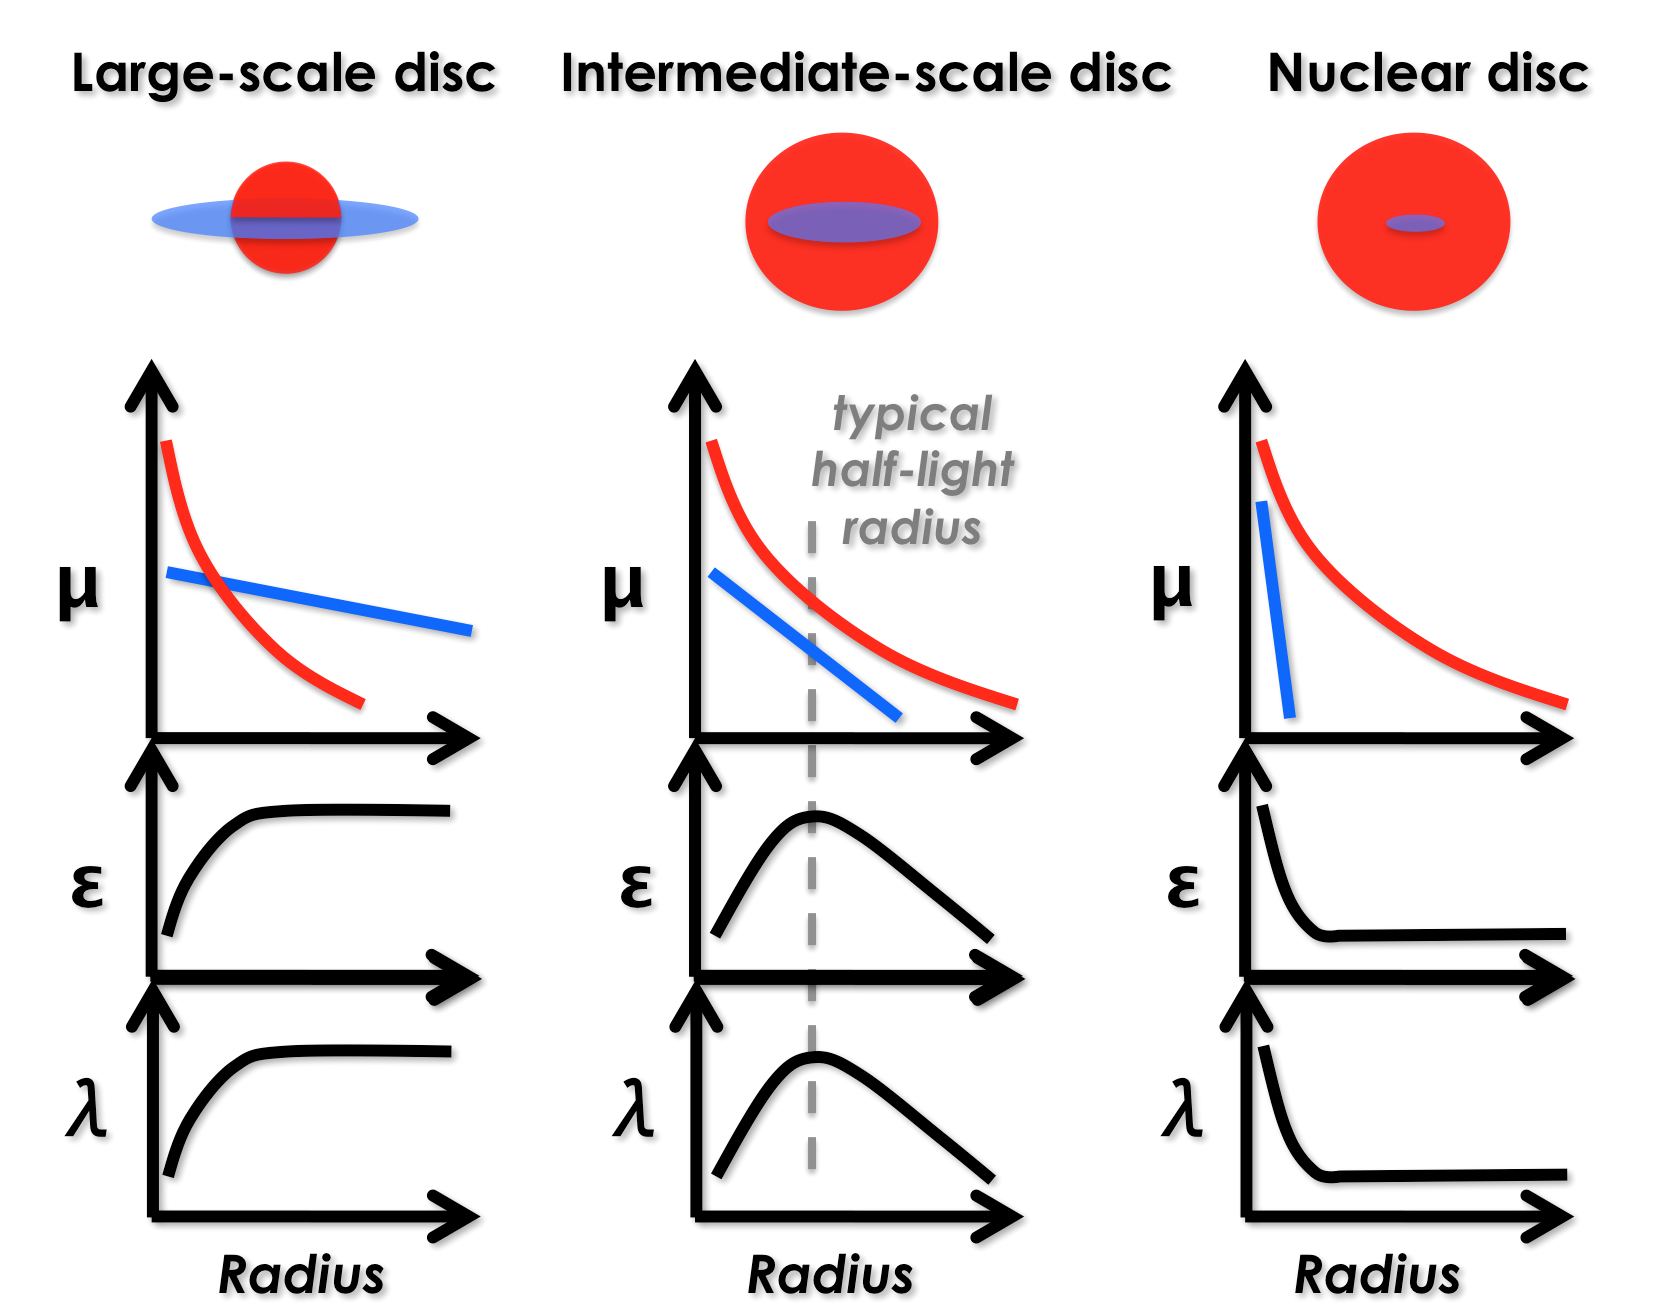
\includegraphics[width=\columnwidth]{images/discmodel.eps}
\caption{Illustration of the spheroid/disc decomposition of the one-dimensional surface brightness profile, $\mu$, 
the ellipticity profile, $\epsilon$, and the specific angular momentum profile, $\lambda$,
for the three prototype early-type galaxy sub-classes. 
In the flux decompositions, the spheroid (or bulge) and the disc are shown with the red and blue color, respectively. 
The left panel shows a lenticular galaxy, composed of a bulge encased in a large-scale disc. 
The right panel displays an elliptical galaxy with (an optional) nuclear stellar disc. 
The middle panel presents an early-type galaxy with an intermediate-sized disc embedded in the spheroid. 
We refer to the last case as an ellicular galaxy.}
\label{fig:model}
\end{center}
\end{figure}


\section{Intermediate-scale disc galaxies}
\label{sec:gal}
Three examples of ellicular galaxies are Mrk 1216, NGC 1332, and NGC 3115. 
In the following Sections, we present a photometric analysis of these three galaxies, 
and we compare our results with the kinematical analysis (when) available from the literature. 
For the galaxies NGC 1332 and NGC 3115, we used $3.6~\rm \mu m$ images obtained with the InfraRed Array Camera (IRAC) 
onboard the \emph{Spitzer Space Telescope}. 
For the galaxy Mrk 1216, we used an archived Hubble Space Telescope (\emph{HST}) image  
taken with the Wide Field Camera 3 (WFC3) and the near-infrared \emph{F160W} filter ($H$-band). 
Our galaxy decomposition technique is extensively described in Savorgnan \& Graham (\emph{submitted}).
Briefly, the galaxy images were background-subtracted, and masks for contaminating sources were created. 
The one-dimensional Point Spread Function (PSF) was characterized using a Gaussian profile for the \emph{HST} observation 
and a \cite{moffat1969} profile for the \emph{Spitzer} observations.
We performed an isophotal analysis of the galaxies using the IRAF\footnote{IRAF 
is the Image Reduction and Analysis Facility, distributed by the National Optical Astronomy Observatory, 
which is operated by the Association of Universities for Research in Astronomy (AURA) 
under cooperative agreement with the National Science Foundation.} task {\tt ellipse}\footnote{Our analysis 
was performed before {\tt isofit} \citep{ciambur2015} was conceived or available. 
After {\tt isofit} was recently developed and implemented in IRAF, 
we employed it to re-extract the surface brightness profiles of the galaxies NGC 1332 and NGC 3115. 
We then repeated the analysis and checked that this change does not significantly alter our results. 
In fact, although {\tt isofit} provides a more accurate description of the isophotes in presence of an inclined disc, 
the discs of NGC 1332 and NGC 3115 are relatively faint compared to the spheroidal components, 
therefore the differences between the light profile obtained with {\tt ellipse} and that obtained with {\tt isofit} are small. } 
\citep{taskellipse}. 
The galaxy isophotes were modelled with a series of concentric ellipses, 
allowing the ellipticity, the position angle and the amplitude of the fourth harmonic to vary with radius.  
The decomposition of the surface brightness profiles was performed with software written by G. Savorgnan.
We modelled the light profiles with a combination of PSF-convolved analytic functions, 
using one function per galaxy component. 


\subsection{NGC 3115}
The presence of a disc in NGC 3115 is obvious due to its edge-on orientation (Figure \ref{fig:n3115}). 
Less obvious is the extent of such disc, if one only relies on a visual inspection of the galaxy image. 
The ellipticity profile is consistent with the presence of an intermediate-scale disc. 
Moreover, the kinematics of NGC 3115 \citep{arnold2011n3115} also disprove the presence of a large scale disc, 
because the galaxy is rapidly rotating only within two galaxy half-light radii ($\sim 2 \times 50~\rm arcsec$), 
whereas the rotation significantly drops at larger radii.  
The unsharp mask of NGC 3115 (Figure \ref{fig:n3115}) betrays the presence of a fain edge-on nuclear ring, 
which can also be spotted as a small peak in the ellipticity profile 
(at semimajor-axis lenght $R_{\rm maj} \sim 15~\rm arcsec$).
The spheroidal component of NGC 3115 is well described with a \cite{sersic1963} profile.
The highly inclined intermediate-scale disc is better fit with a $n<1$ S\'ersic profile 
(the S\'ersic index $n$ regulates the curvature of the S\'ersic profile) 
rather than with an exponential function, 
as explained by \cite{pastrav2013a}. 
The nuclear ring is modelled with a Gaussian function. 


\subsection{NGC 1332}
The morphology of NGC 1332 (Figure \ref{fig:n1332}) is very similar to that of NGC 3115, 
with the ellipticity profile indicating the presence of an intermediate-scale disc, 
although in this case no nuclear component was identified from our photometric analysis. 
The authors of this paper were not able to find any extended kinematic profile or map 
for this galaxy in the literature. 
The data within the innermost $6~\rm arcsec$ were excluded from the fit 
because possibly affected by the presence of a partially depleted core.
The surface brightness profile of NGC 1332 is well described with a S\'ersic-spheroid plus
a $n<1$ S\'ersic-disc. 
Our galaxy decomposition suggests that NGC 1332 is a spheroid-dominated galaxy, 
with a spheroid-to-total ratio of $0.95$.
\cite{rusli2011} did not identify the extent of the intermediate-scale disc, 
and proposed a model featuring a S\'ersic-bulge and a large-scale exponential-disc, 
with a spheroid-to-total ratio of $0.43$.
Based on such bulge-disc decomposition, they concluded that NGC 1332 is a disc dominated lenticular galaxy 
which is displaced from the (black hole mass)-(spheroid luminosity) correlation of \cite{marconihunt2003} 
by an order of magnitude along the black hole mass direction. 
However, in Section \ref{sec:mm} we show that, according to our decomposition, 
NGC 1332 lies within the $1\sigma$ scatter about the (black hole mass)-(spheroid stellar mass) correlation 
for early-type galaxies. 


\subsection{Mrk 1216}
Although the disc in the galaxy Mrk 1216 is not immediately apparent from the image (Figure \ref{fig:m1216}), 
the velocity map \citep{yildirim2015} proves the presence of a fast rotating component 
at least within three galaxy half-light radii ($\sim 3 \times 5~\rm arcsec$). 
The ellipticity profile (Figure \ref{fig:m1216}) indicates the presence of an intermediate-scale disc. 
In addition, a nuclear disc is identified from the change in slope of the ellipticity profile ($R_{\rm maj} \sim 1 - 2 \rm~arcsec$) 
and from a clear feature in the fourth harmonic profile (not shown here). 
We modelled the surface brightness profile of Mrk 1216 (Figure \ref{fig:m1216}) with a S\'ersic-spheroid, 
an intermediate-sized exponential-disc, and a nuclear exponential-disc. 

\subsection{Other galaxies}
Our models with an intermediate-sized disc embedded within a larger spheroidal component, 
plus an additional nuclear component when one is present, 
match the observed light distribution, and explain both the extended kinematic maps (when available, \citealt{arnold2014}) and the ellipticity profiles, 
of other galaxies for which a direct measurement of their central supermassive black hole mass is available: 
NGC 821; NGC 1271; NGC 1277; NGC 3377; and NGC 4697. 
Our isophotal analysis and galaxy decompositions for NGC 1271 and NGC 1277 will be presented in 
Graham, Savorgnan \& Ciambur (\emph{in prep.}) and Graham et al.~(\emph{in prep.}), respectively, 
while the galaxies NGC 821, NGC 3377 and NGC 4697 have been analysed in Savorgnan \& Graham (\emph{submitted}). 


\begin{figure}
\begin{center}
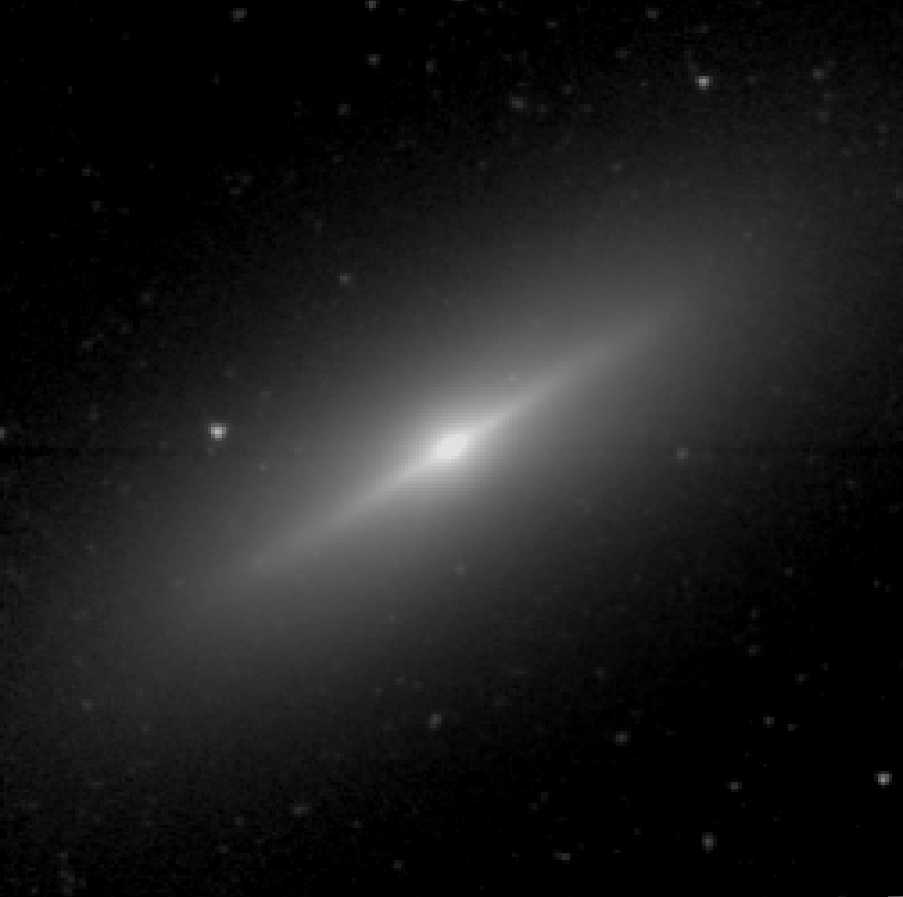
\includegraphics[width=0.49\columnwidth]{images/n3115_image.jpeg}
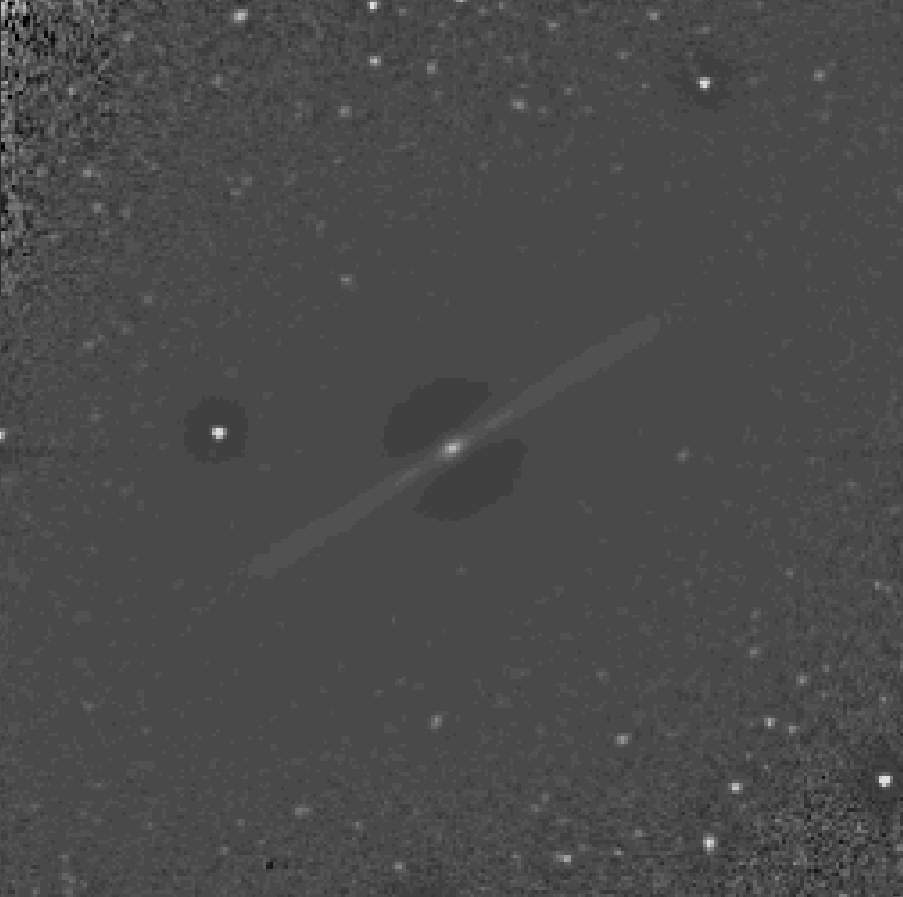
\includegraphics[width=0.49\columnwidth]{images/n3115_unsharp.jpeg} \\
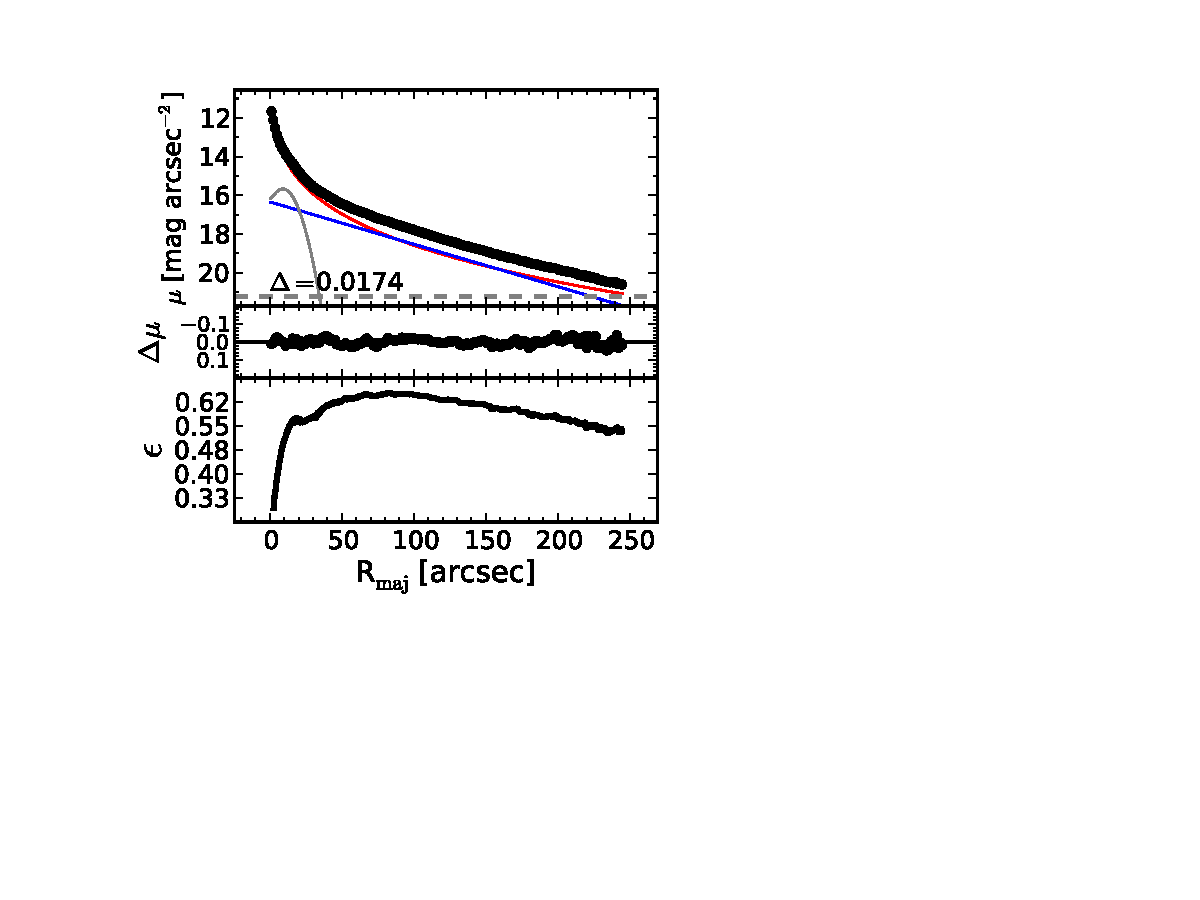
\includegraphics[width=1.05\columnwidth]{images/n3115_decomposition.pdf}
\caption{The galaxy NGC 3115. 
The top panels are the \emph{Spitzer}/IRAC $3.6~\rm \mu m$ image (left) and its unsharp mask (right), 
obtained by dividing the image by a Gaussian-smoothed version of itself. 
The bottom plots display the best-fit model of the surface brightness profile, $\mu$, 
and the ellipticity profile, $\epsilon$, 
along the major-axis, $R_{\rm maj}$. 
The black points are the observed data, which extend out to five galaxy half-light radii ($\sim 5 \times 50~\rm arcsec$). 
The color lines represent the individual (PSF-convolved) model components: 
red = S\'ersic (spheroid), blue = S\'ersic (disc), gray = Gaussian ring. 
The residual profile (data $-$ model) is shown as $\Delta \mu$. 
The horizontal gray dashed line corresponds to an intensity equal to three times the root mean square of the sky background fluctuations. 
$\Delta$ denotes the root mean square scatter of the fit in units of $\rm mag~arcsec^{-2}$. }
\label{fig:n3115}
\end{center}
\end{figure}

\begin{figure}
\begin{center}
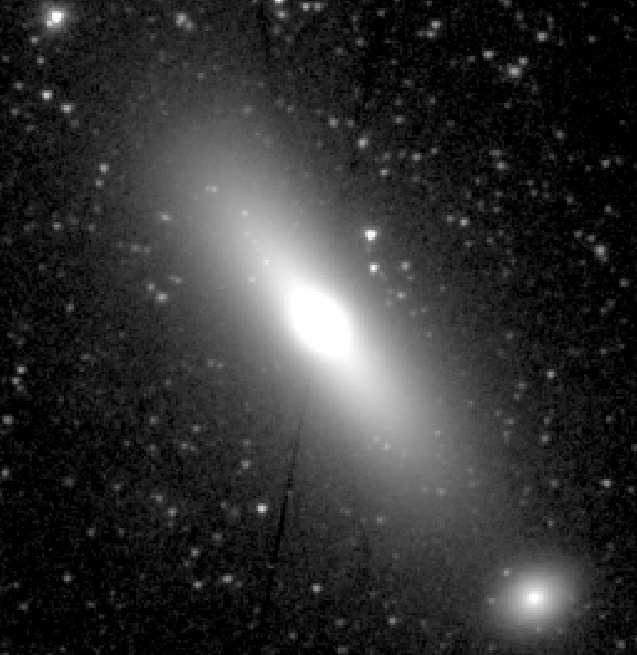
\includegraphics[width=0.49\columnwidth]{images/n1332_image}
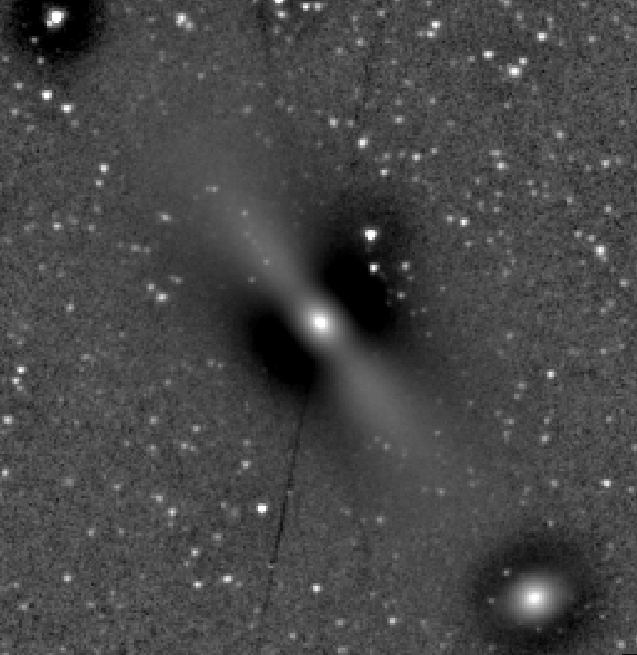
\includegraphics[width=0.49\columnwidth]{images/n1332_unsharp} \\
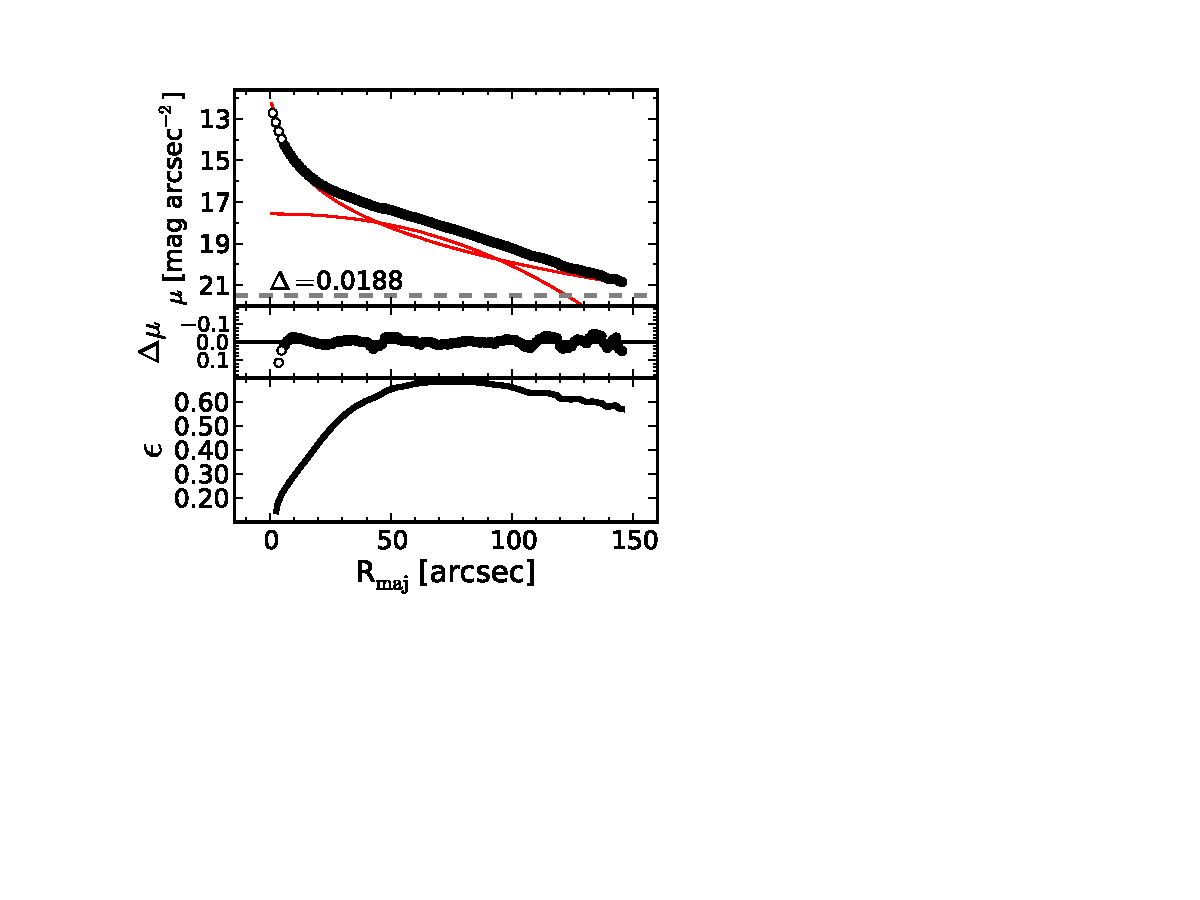
\includegraphics[width=1.03\columnwidth]{images/n1332_decomposition.pdf}
\caption{The galaxy NGC 1332. 
The top panels are the \emph{Spitzer}/IRAC $3.6~\rm \mu m$ image (left) and its unsharp mask (right), 
obtained by dividing the image by a Gaussian-smoothed version of itself. 
The bottom plots display the best-fit model of the surface brightness profile, $\mu$, 
and the ellipticity profile, $\epsilon$, 
along the major-axis, $R_{\rm maj}$. 
The black points are the observed data, which extend out to seven galaxy half-light radii ($\sim 7 \times 20~\rm arcsec$). 
The empty points are data excluded from the fit.   
The color lines represent the individual (PSF-convolved) model components: 
red = S\'ersic (spheroid), blue = S\'ersic (disc). 
The residual profile (data $-$ model) is shown as $\Delta \mu$. 
The horizontal gray dashed line corresponds to an intensity equal to three times the root mean square of the sky background fluctuations. 
$\Delta$ denotes the root mean square scatter of the fit in units of $\rm mag~arcsec^{-2}$.
}
\label{fig:n1332}
\end{center}
\end{figure}

\begin{figure}
\begin{center}
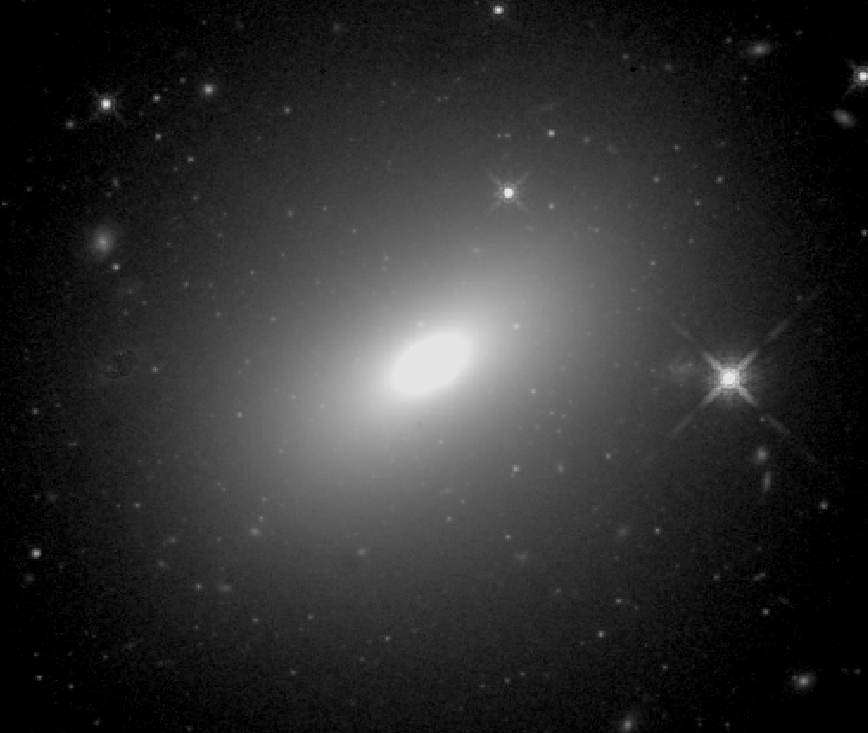
\includegraphics[width=0.49\columnwidth]{images/mrk1216_image.jpeg}
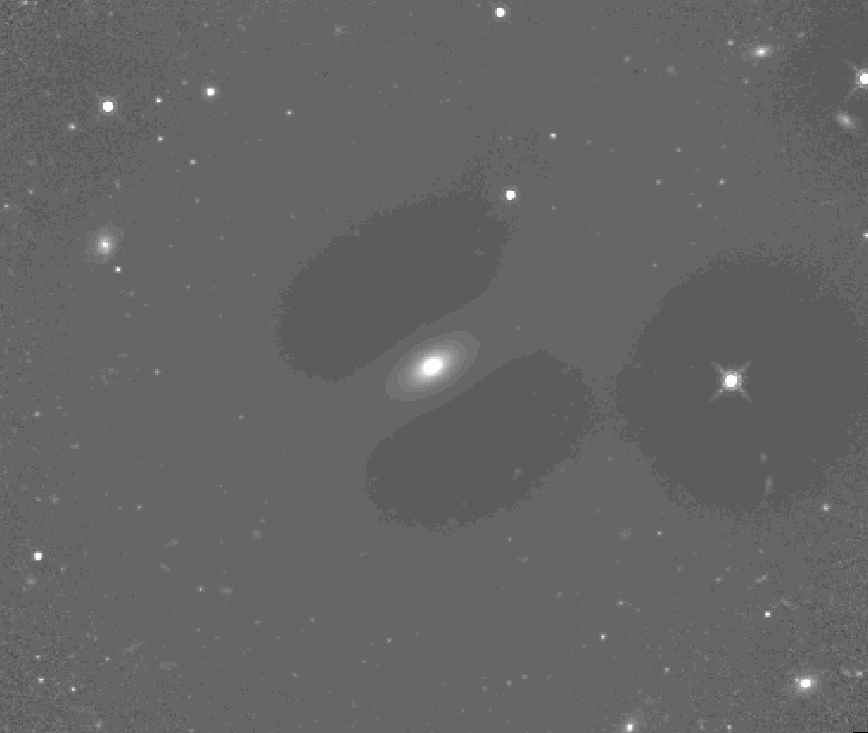
\includegraphics[width=0.49\columnwidth]{images/mrk1216_unsharp.jpeg} \\
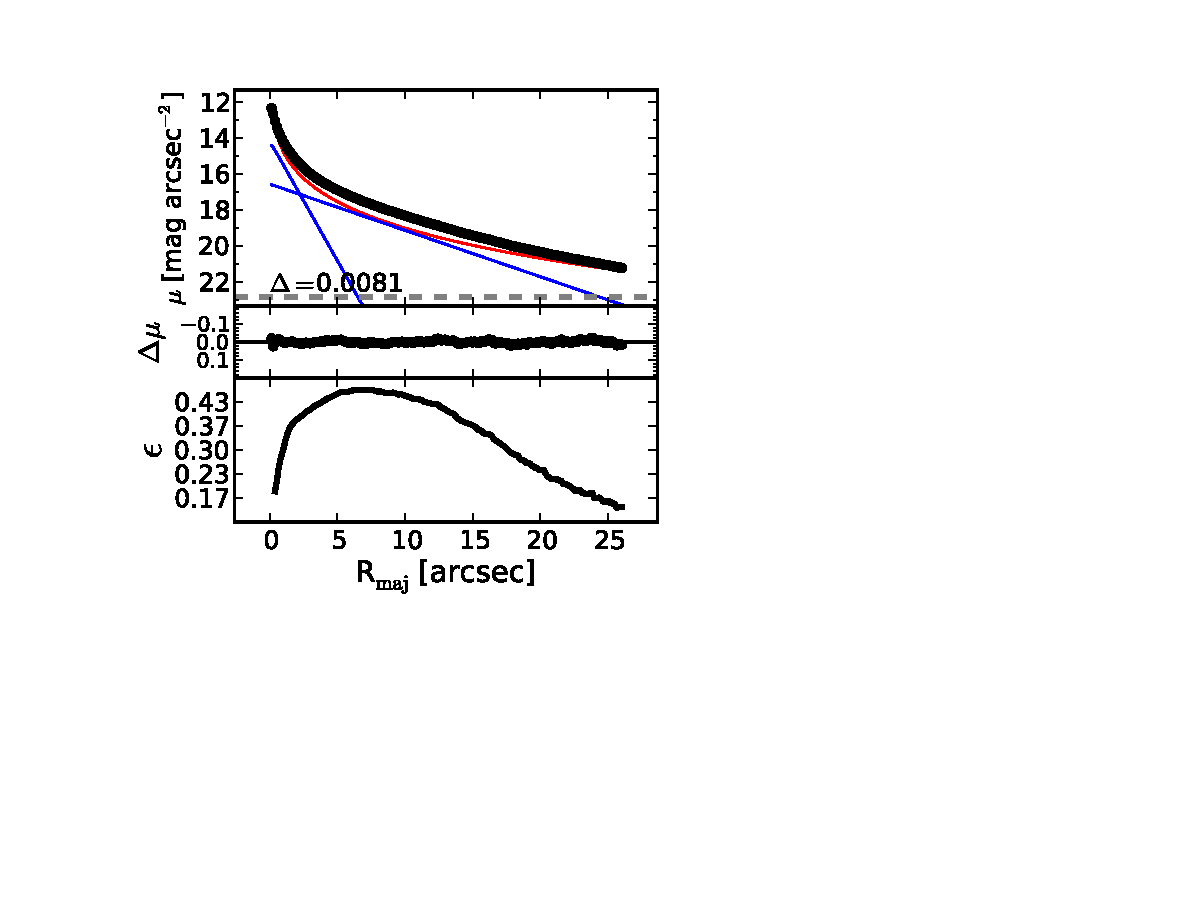
\includegraphics[width=1.05\columnwidth]{images/mrk1216_decomposition.pdf}
\caption{The galaxy Mrk 1216. 
The top panels are the \emph{HST}/WFC3 \emph{F160W} image (left) and its unsharp mask (right), 
obtained by dividing the image by a Gaussian-smoothed version of itself. 
The bottom plots display the best-fit model of the surface brightness profile, $\mu$, 
and the ellipticity profile, $\epsilon$, 
along the major-axis, $R_{\rm maj}$. 
The black points are the observed data, which extend out to five galaxy half-light radii ($\sim 5 \times 5~\rm arcsec$).
The color lines represent the individual (PSF-convolved) model components: 
red = S\'ersic (spheroid), blue = exponential (disc). 
The residual profile (data $-$ model) is shown as $\Delta \mu$. 
The horizontal gray dashed line corresponds to an intensity equal to three times the root mean square of the sky background fluctuations. 
$\Delta$ denotes the root mean square scatter of the fit in units of $\rm mag~arcsec^{-2}$.
}
\label{fig:m1216}
\end{center}
\end{figure}



\section{Implications}
\label{sec:impl}
Past models that ``forcedly'' described ellicular galaxies using an inner bulge 
encased within a large-scale disc 
commonly required the addition of an extended envelope or halo to account for the outer portion of the spheroid. 
Such three-component models (bulge + disc + envelope) typically reduce the spheroid luminosity by a factor of $3-4$, 
and underestimate the size of the spheroid by a factor of $6-10$, 
although more ``extreme'' cases can be found. \\
\cite{lasker2014data} fit the galaxy NGC 3115 with a bulge + disc + envelope, 
and measured a bulge half-light radius of $3.9~\rm arcsec$ and a bulge-to-total ratio of $0.12$; 
we described this galaxy using a spheroid + intermediate-scale disc + nuclear ring, 
and obtained a spheroid half-light radius of $43.6~\rm arcsec$ and a spheroid-to-total ratio of $0.85$. \\
\cite{vandenbosch2012} proposed a model for the galaxy NGC 1277 with a bulge + disc + nuclear source + envelope, 
which gives a bulge half-light radius of $0.9~\rm arcsec$ and a bulge-to-total ratio of $0.24$; 
our model consists of a spheroid + intermediate-scale disc + nuclear component, 
and produces a spheroid half-light radius of $6.0~\rm arcsec$ and a spheroid-to-total ratio of $0.79$. \\
\cite{lasker2014data} modelled the galaxy NGC 3377 with a bulge + nuclear disc + disc + envelope, 
and obtained a bulge half-light radius of $10.1~\rm arcsec$ and a bulge-to-total ratio of $0.35$; 
our model with a spheroid + intermediate-scale disc + nuclear disc 
returns a spheroid half-light radius of $61.8~\rm arcsec$ and a spheroid-to-total ratio of $0.94$. \\
\cite{lasker2014data} decomposed the galaxy NGC 821 into a bulge + disc + envelope, 
and measured a bulge half-light radius of $3.8~\rm arcsec$ and a bulge-to-total ratio of $0.19$; 
our decomposition consists of a spheroid + intermediate-scale disc, 
with a spheroid half-light radius of $36.5~\rm arcsec$ and a spheroid-to-total ratio of $0.79$. \\
The galaxy NGC 4697 represents an ``extreme'' case. 
\cite{lasker2014data} fit this galaxy with a bulge + nuclear source + disc + envelope, 
and obtained a bulge half-light radius of $6.3~\rm arcsec$ and a bulge-to-total ratio of $0.08$; 
we described NGC 4697 using a spheroid + intermediate-scale disc + inner disc model, 
and measured a spheroid half-light radius of $239.3~\rm arcsec$ and a spheroid-to-total ratio of $0.89$.


\subsection{The black hole -- spheroid correlation}
\label{sec:mm}
Inaccurate measurements of the spheroid-to-total ratio of galaxies can impact galaxy scaling relations. 
Recently, a handful of ellicular galaxies have been claimed to host \emph{{\"u}ber-massive} black holes, 
i.e.~their central supermassive black hole has been reported to be 
over-massive compared to expectations from the spheroid luminosity (or stellar mass).
This is the case for the galaxies Mrk 1216 (for which only an upper limit on its black hole mass has been published, 
\citealt{yildirim2015}), NGC 1271 \citep{walsh2015}, 
NGC 1277 \citep{vandenbosch2012,yildirim2015} and NGC 1332 \citep{rusli2011}.
In addition to these, also the elliptical galaxy NGC 4291 has been claimed to be a $\sim$$3.6\sigma$ outlier 
above the (black hole mass)-(spheroid mass) scaling relation \citep{bogdan2012}. 
Obviously, having both the black hole mass and the spheroid mass correct is important 
for placing systems in the (black hole mass)-(spheroid mass) diagram. 
\emph{For early-type galaxies, the spheroid luminosity and the galaxy luminosity 
can be used to predict the black hole mass with the same level of accuracy\footnote{Note that 
\cite{lasker2014anal} reported that the spheroid luminosity and the galaxy luminosity are equally good tracers of the black hole mass 
irrespective of the galaxy morphological type, but their sample of 35 galaxies contained only 4 spiral galaxies. 
However, using a sample of 45 early-type and 17 spiral galaxies, 
Savorgnan et al.~(\emph{submitted}) shows that, when considering all galaxies irrespective of their morphological type, 
the correlation of the black hole mass with the spheroid luminosity is better than that with the galaxy luminosity.} 
(Savorgnan et al.~submitted). 
If a galaxy hosts a black hole that is over-massive compared to expectations from the spheroid luminosity, 
but whose mass is normal compared to expectations from the galaxy luminosity, 
one should wonder whether the spheroid luminosity might have been underestimated 
due to an inaccurate spheroid/disc decomposition. }
Indeed, none of the five galaxies mentioned before (Mrk 1216, NGC 1271, NGC 1277, NGC 1332, and NGC 4291) is a noticeable outlier 
in the (black hole mass)-(galaxy luminosity) diagram. 
In Figure \ref{fig:mm} we show the location of these five galaxies in the (black hole mass)-(spheroid stellar mass) diagram 
for early-type galaxies of Savorgnan et al.~(\emph{submitted}). 
Figure 4 was populated using a galaxy decomposition technique extensively described in Savorgnan \& Graham (\emph{submitted}). 
Briefly, we obtained Spitzer/IRAC $3.6~\rm \mu m$ images for 45 early-type galaxies 
which already had a dynamical detection of their black hole mass. 
We modelled their one-dimensional surface brightness profiles with a combination of analytic functions, using one function per galaxy component. 
Spheroid luminosities were converted into stellar masses using individual, but almost constant mass-to-light ratios ($\sim$$0.6$, \citealt{meidt2014-MNRAS}). 
In addition, we show the galaxies Mrk 1216, NGC 1271 and NGC 1277, which were not a part of the original sample of 45.
For the galaxy NGC 1271, we use the black hole mass measurement and the mass-to-light ratio obtained by \cite{walsh2015}. 
The luminosity of the spheroidal component of this galaxy comes from the one-dimensional spheroid/disc decomposition 
of Graham, Savorgnan \& Ciambur (\emph{in prep.}),  
who used an archived \emph{HST} image taken with the WFC3 and the near-infrared \emph{F160W} filter. 
For the galaxy NGC 1277, we use the black hole mass measurement obtained by \cite{vandenbosch2012} 
and the mass-to-light ratio obtained by \cite{martinnavarro2015}. 
The luminosity of the spheroidal component of this galaxy comes from the one-dimensional spheroid/disc decomposition of Graham et al.~(\emph{in prep.}), 
who used an archived \emph{HST} image taken with the Advanced Camera for Surveys (\emph{ACS}) and the \emph{F550M} filter. 
For the galaxy Mrk 1216, we use the upper limit on the black hole mass and the mass-to-light ratio obtained by \cite{yildirim2015}. 
The luminosity of the spheroidal component of this galaxy comes from our one-dimensional spheroid/disc decomposition (Figure \ref{fig:m1216}).
For the first time, Figure \ref{fig:mm} reveals that when these five galaxies are properly modeled, 
they no longer appear as extreme outliers above the (black hole mass)-(spheroid stellar mass) correlation for early-type galaxies, 
i.e.~they all reside well within a $3\sigma$ deviation from the correlation.

%{\bf change: This not only nullifies the need for invoking different evolutionary scenarios for these galaxies 
%but it strengthens the significance of the observed (black hole mass)-(spheroid mass) correlation 
%and confirms its importance as a fundamental ingredient for theoretical and semi-analytic models 
%used to describe the coevolution of spheroids and their central supermassive black holes. }

\subsection{Origin of compact massive galaxies}
Acknowledging the correct structure of ellicular galaxies is also important to properly understand their origin. 
According to the current paradigm of cosmological structure evolution, 
the genesis of massive early-type galaxies is characterized by two distinct phases: ``in-situ'' and ``ex-situ''. 
The first phase takes place in a young Universe (within its first $4~\rm Gyr$), 
when cold gas inflows produced short and intense bursts of star formation that created the cores of galaxies. 
These naked and compact cores, named ``red nuggets'' \citep{damjanov2009}, have been observed at high-redshift with sizes of $1-2~\rm kpc$ \citep{vandokkum2008}.
In the second phase (last $10~\rm Gyr$), stellar discs and stellar envelopes 
were accreted around these primordial galaxy cores and assembled the external parts of galaxies on scales of $2-20~\rm kpc$. 
Today's Universe is populated by an abundance of compact, massive spheroids, 
with the same physical properties -- mass and compactness -- as the high-redshift red nuggets \citep{GDS2015}. 
Some of these local compact massive spheroids are encased within a large-scale disc, 
that is to say they are the bulges of some lenticular and spiral galaxies. 
Over the last $10~\rm Gyr$ their spheroids have evolved by growing a relatively flat disc -- 
rather than a three-dimensional envelope -- 
which has increased the galaxy size but preserved the bulge compactness. 
The other compact massive spheroids of today's Universe belong to some ellicular galaxies. 
Indeed, Mrk 1216, NGC 1271, NGC 1277, NGC 1332, and NGC 3115 are all local compact ellicular galaxies 
with purely old ($>10~\rm Gyr$) stellar populations. 
These galaxies have undergone the lowest degree of disc growth. \\
In addition to the observational clues as to the actual physical components in ellicular galaxies, 
one can reason on other grounds as to why these compact galaxies are not comprised of an inner bulge 
plus large-scale disc plus outer envelope. 
If they were such three-component systems, then one would have two possibilities. 
The first possibility is that these galaxies were already fully assembled $10~\rm Gyr$ ago; 
this would explain their old stellar populations, 
but it would also imply that their discs and envelopes had already formed during the first $4~\rm Gyr$ of the Universe, 
in disagreement with the current cosmological picture. 
The second possibility is that only their inner bulges (with sizes of $0.1-0.2~\rm kpc$, 
according to past decompositions) originated in the first $4~\rm Gyr$ 
and they subsequently accreted a substantial disc and envelope. 
If this was correct, then we would observe high-redshift, star-like, naked bulges with stellar masses 
within a factor of a few times the currently observed red nuggets but sizes which are $10$ times smaller. 
However, a dramatically different expectation is reached 
if one considers these galaxies as spheroid-dominated systems with an intermediate-scale disc; 
in this case, both the galaxy size and the spheroid size are compact ($1-2~\rm kpc$). 
This implies that, among the local descendants of the high-redshift red nuggets, 
the compact ellicular galaxies have undergone the lowest degree of disc growth. 
That is, the bulk of a compact ellicular galaxy quickly assembled ``in-situ'' in a very young Universe 
and experienced very little evolution over the last $10~\rm Gyr$.

\begin{figure}
\begin{center}
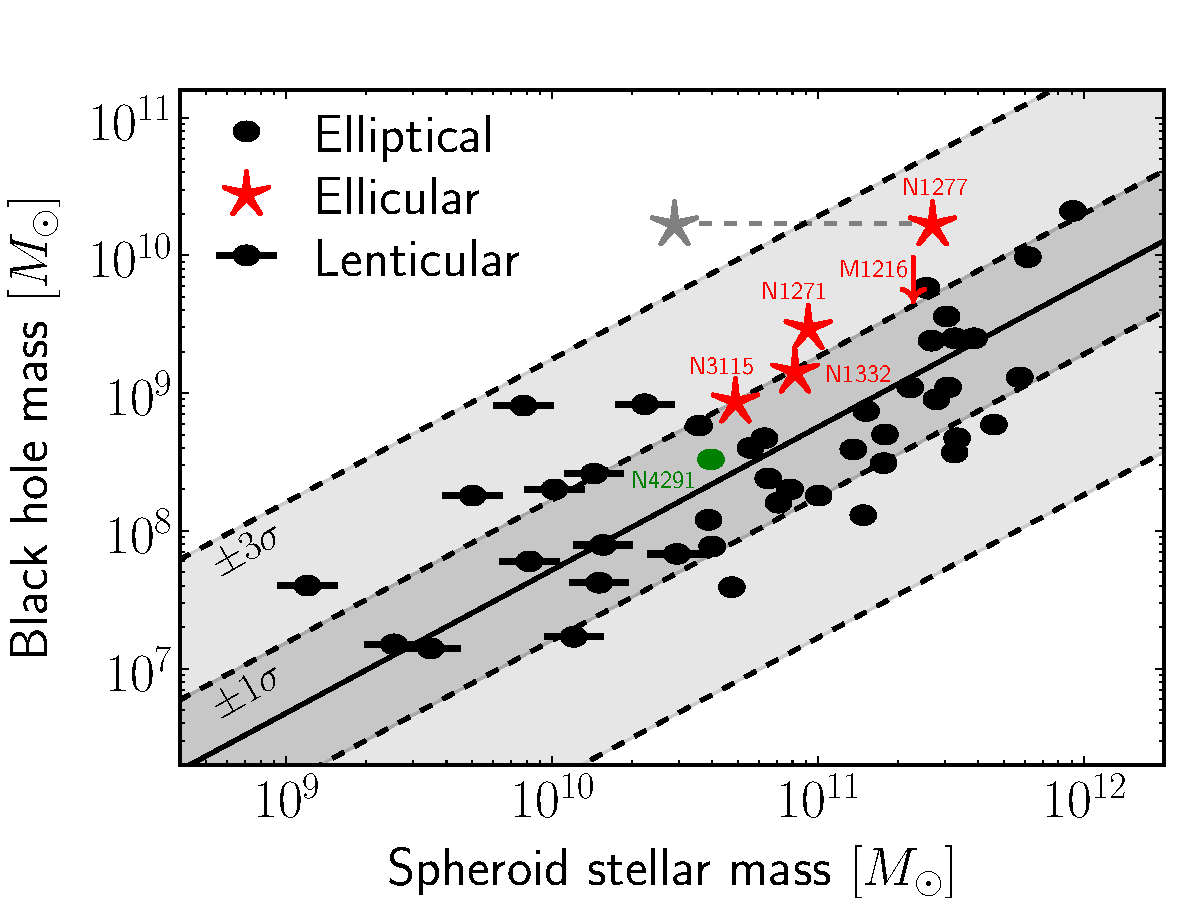
\includegraphics[width=\columnwidth]{images/mm.pdf}
\caption{Early-type (elliptical + lenticular) galaxies: 
black hole mass plotted against spheroid stellar mass for 48 galaxies. 
The black solid line is the bisector linear regression for all galaxies except Mrk 1216, NGC 1271 and NGC 1277. 
The dashed lines mark the $1\sigma$ and $3\sigma$ deviations, 
where $\sigma$ ($0.51$ dex) is the total \emph{rms} scatter about the correlation in the black hole mass direction. 
The red stars mark four intermediate-scale disc galaxies (Mrk 1216, NGC 1271, NGC 1277 and NGC 1332) and one elliptical galaxy (NGC 4291) 
that were claimed to be extreme outliers in this diagram. 
All five reside within a $3\sigma$ deviation from the correlation when using their correct spheroid mass. 
For NGC 1277, we show the previously reported spheroid stellar mass \citep{vandenbosch2012} in gray. 
The green color is used to show the location of four other intermediate-scale disc galaxies mentioned in Section \ref{sec:impl}.}
\label{fig:mm}
\end{center}
\end{figure}

\subsection{Ellicular galaxies in the Hubble grid}
The existence of the oft-overlooked, intermediate-scale discs presented here exposes a likely continuum of disc sizes in early-type galaxies 
as opposed to a dichotomy of nuclear discs versus large-scale discs. 
The presence of these intermediate-scale discs also blurs the distinction between elliptical (E) and lenticular (S0) galaxies 
and arguably creates the need for a new subclass which bridges this divide.  
While expanding the galaxy nomenclature beyond ellipticals with possible nuclear discs, and lenticulars with large-scale discs, 
to include something like {\it elliculars} with intermediate-scale discs will be helpful 
for distinguishing among the different early-type galaxies with different disk scale-lengths, 
it should be remembered that just as portions of the electromagnetic spectrum are labelled according to their different wavelengths, 
there is still an underlying continuum.  
Similarly, binning early-type galaxies as either a fast-rotator (FR) or a slow-rotator (SR) can hide the fact that a continuum exists.  
Importantly, in the case of early-type galaxies with intermediate scale discs, 
this particular rotation-classification depends on the galaxy's radial range probed.  
There is thus a need for more than two bins (E vs.~S0, or SR vs.~FR). \\
The existence of intermediate-scale discs is not only important for our understanding of disc growth in general, 
but accounting for such components impacts upon our broader understanding of galaxy structure.  
It has recently been argued \citep{graham2014review} that the classification scheme for elliptical galaxies 
should not be their apparent axis ratio as seen on the plane of the sky, 
but rather early-type galaxies should be quantified by their spheroid-to-total flux ratio, 
with a continuum from pure elliptical galaxies to disc-dominated lenticular galaxies.   
While spiral galaxies display a range of spheroid-to-total flux ratios from 0 to $\sim$3/4, 
lenticular galaxies display a range from $\sim$3/4 to $\sim$0.1 (see \citealt{laurikainen2010}).   
The spheroid-to-total flux ratio is an important quantity, and its broad range observed in lenticular galaxies 
has led to a resurgence of \citeauthor{vandenbergh1976}'s (\citeyear{vandenbergh1976}) Hubble comb, 
in which both late-type galaxies (i.e.~spiral galaxies) and lenticular galaxies form the arms of an expanded Hubble tuning fork, 
with an additional arm for disc galaxies hosting anaemic spiral patterns (see \citealt{cappellari2011kmdr-MNRAS} and \citealt{kormendybender2012}).  
However because every spiral Hubble type (e.g.~Sa, Sb, Sc) has a broad range of spheroid-to-total ratio 
(e.g.~\citealt{grahamworley2008}, and references therein), 
and because this information is not captured by the Hubble comb, 
a grid of spiral type (predominantly determined by the spiral arms) versus spheroid-to-total ratio is also useful for classifying galaxies.   
In Figure \ref{fig:grid} we show the location of galaxies with intermediate-scale discs in such a Hubble grid \citep{graham2014review}, 
revealing how they are related to the other galaxies.  
Aside from the pure elliptical galaxies, each galaxy type displays a range of spheroid-to-total flux ratio.  
Rather than a scheme in which the spiral morphological type (a, b, c, etc.) changes if the spheroid-to-total ratio changes (as in the Hubble comb), 
here the galaxy type is linked to the nature and winding of the spiral arms which has been the primary criteria used 
to classify spiral galaxies over the last half century \citep{sandage1961}.

\begin{figure}[h]
\begin{center}
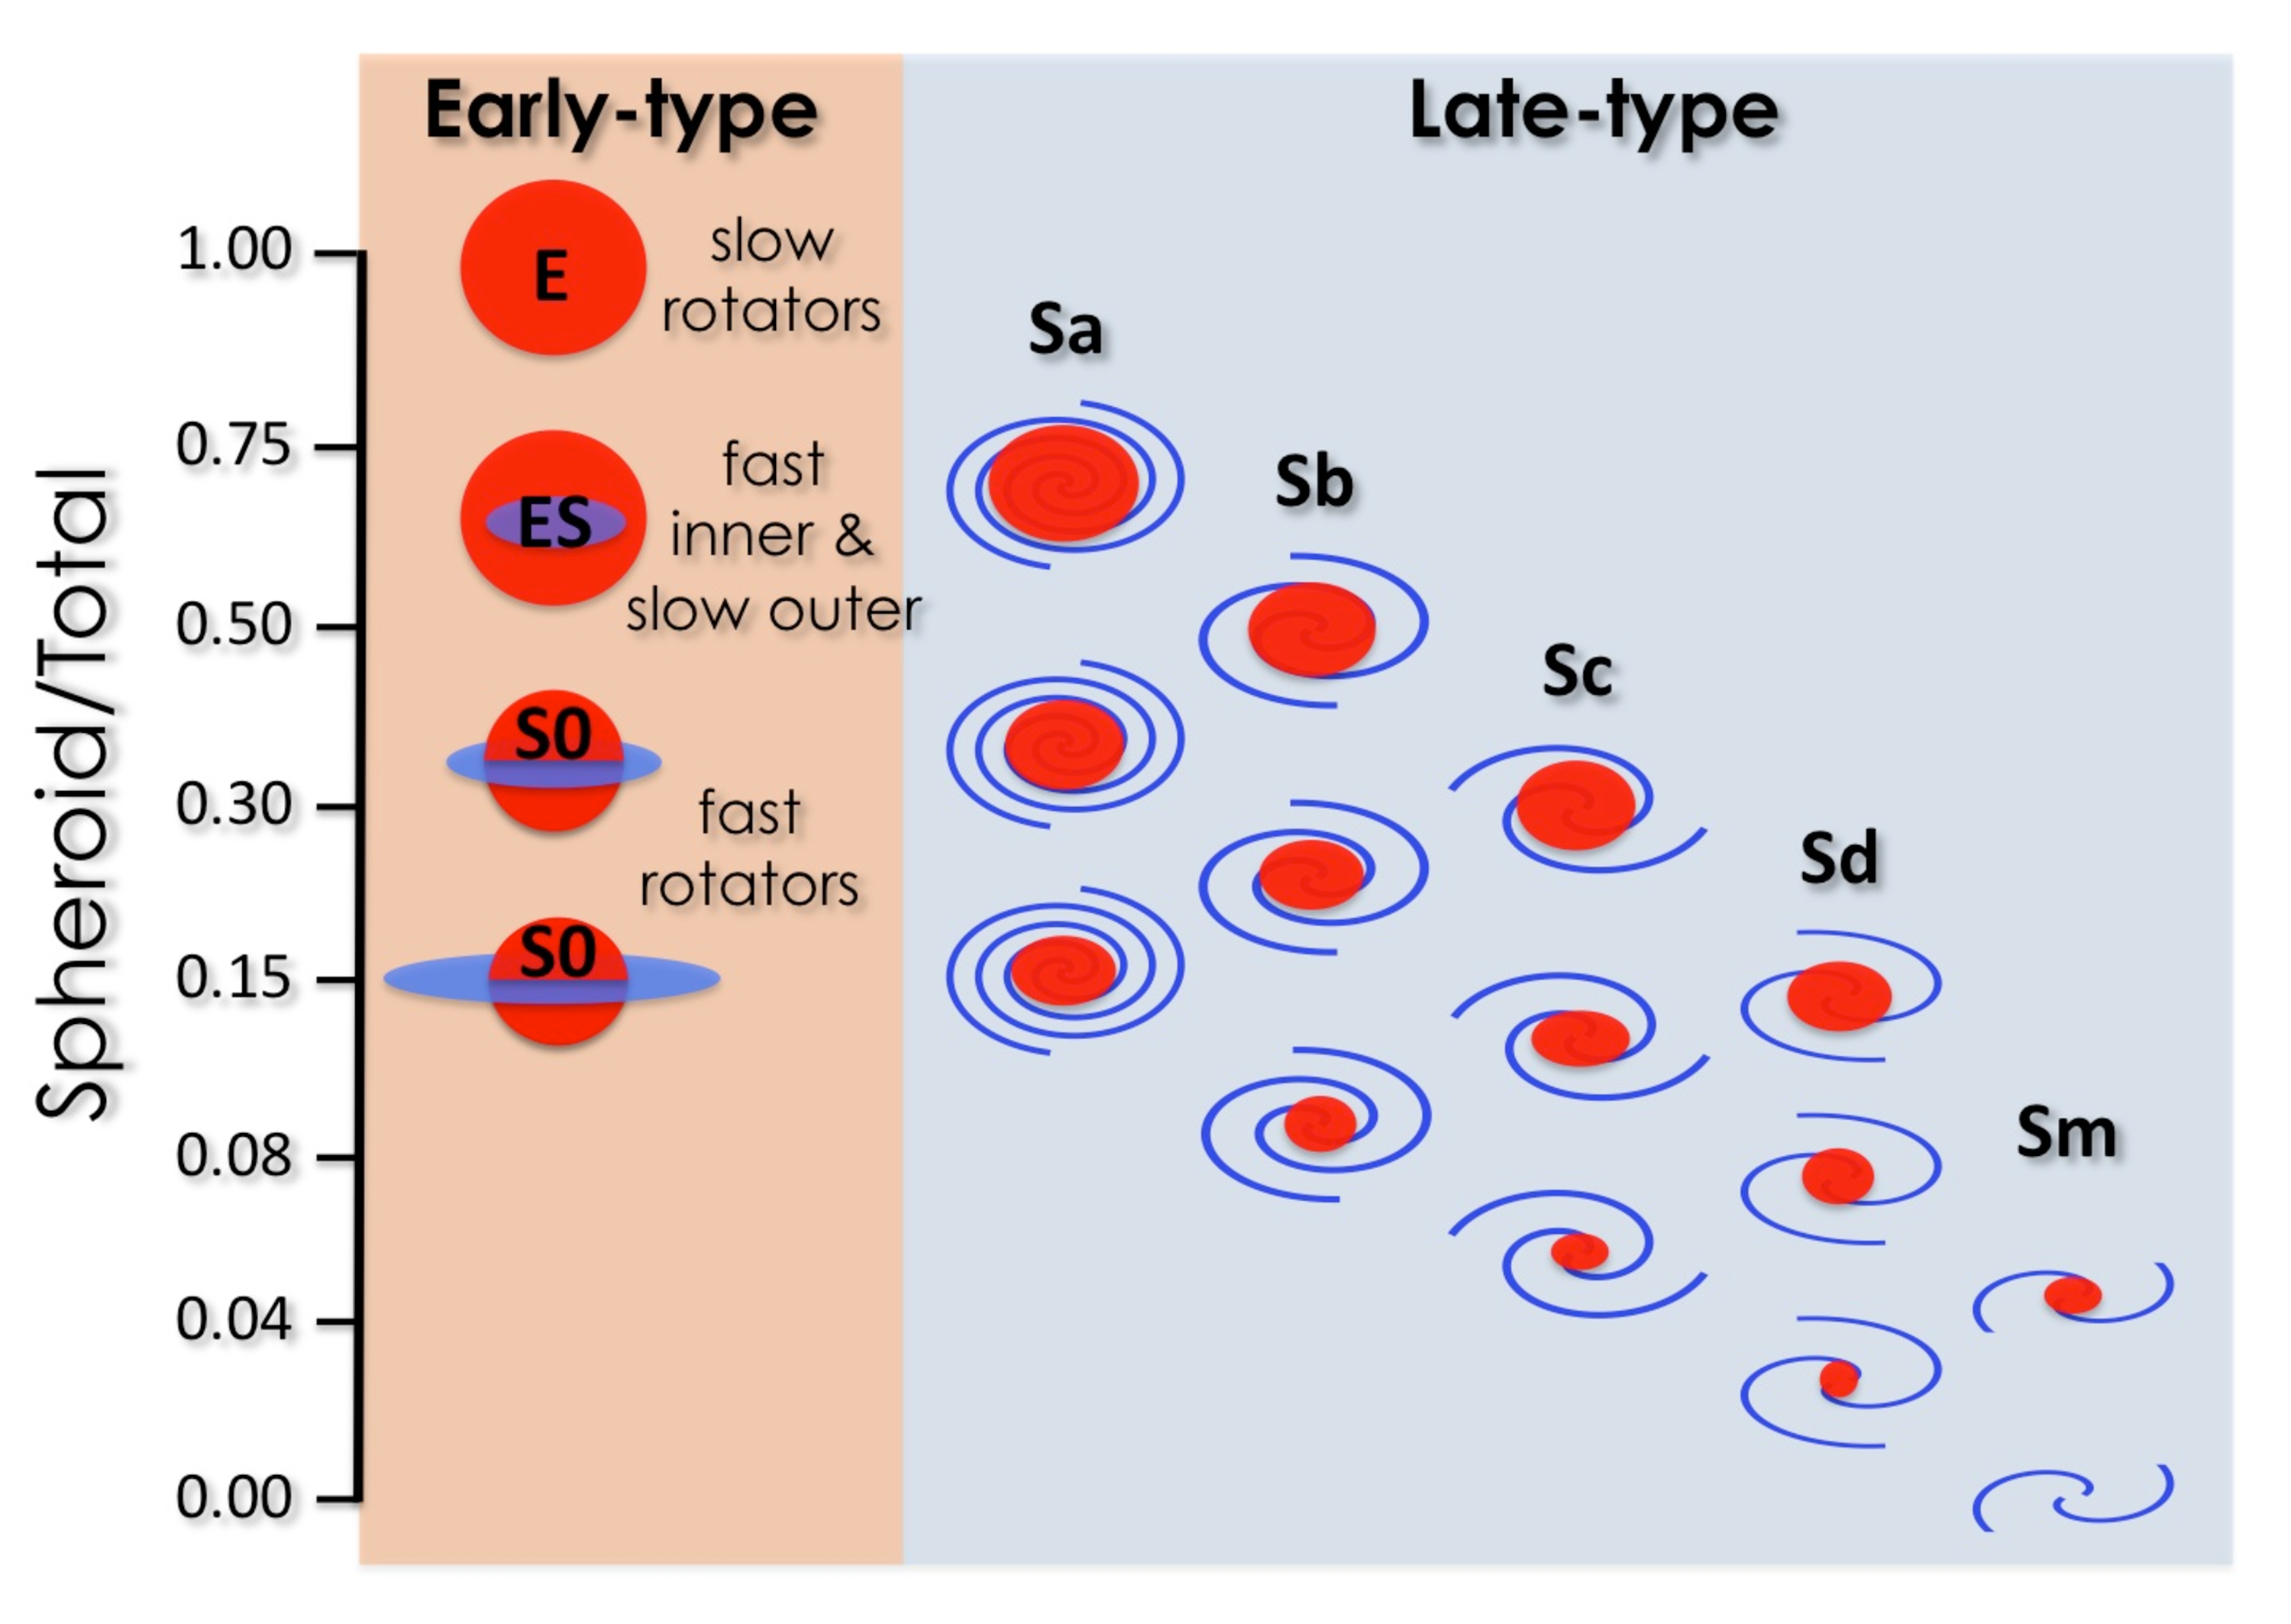
\includegraphics[width=\columnwidth]{images/Hubble-grid-2/Hubblegrid.pdf}
\caption{The Hubble grid \citep{graham2014review}, 
which uses the mean pitch angle of the arms in spiral galaxies to define their morphological type. 
Ellicular (ES) galaxies are intermediate between elliptical (E) and lenticular (S0) galaxies. }
\label{fig:grid}
\end{center}
\end{figure}

\section{Acknowledgments}
% referee thank you!!
This research was supported by Australian Research Council funding through grant FT110100263. 
GS is grateful to Matteo Fossati, Luca Cortese and Giuseppe Gavazzi for useful comments and discussion. 
This work is based on observations made with the IRAC instrument \citep{fazio2004IRAC-MNRAS} on-board the Spitzer Space Telescope, 
which is operated by the Jet Propulsion Laboratory, California Institute of Technology under a contract with NASA, 
and also on observations made with the NASA/ESA Hubble Space Telescope, 
and obtained from the Hubble Legacy Archive, 
which is a collaboration between the Space Telescope Science Institute (STScI/NASA), 
the Space Telescope European Coordinating Facility (ST-ECF/ESA) and the Canadian Astronomy Data Centre (CADC/NRC/CSA).
This research has made use of the GOLDMine database \citep{goldmine} and the NASA/IPAC Extragalactic Database (NED) 
which is operated by the Jet Propulsion Laboratory, California Institute of Technology, 
under contract with the National Aeronautics and Space Administration. 

\bibliography{/Users/gsavorgnan/galaxy_vivisection/papers/SMBHbibliography}


\label{lastpage}

\clearpage


\end{document}
